\section{Methoden zur Feature-Auswahl, Hyperparametersuche und Modellauswahl} \label{sec:Meth FeatHypModSelect}
zwischen der Feature-Auswahl, dem Modellauswahl und der Hyperparamtersuche besteht ein enger Zusammenhang. Werden für die Feature-Auswahl modellabhängige Methoden verwendet, wie die Wrapper Methoden, muss ein Modell vorhanden sein, mit welchem sich die Methoden anwenden lassen. Um zwischen unterschiedlichen Modellen auszuwählen auf Basis ihrer Performance, ist eine Einstellung der Hyperparameter notwendig, damit die Modell auch fair bewertet werden. Ein Modell \(A\) wird beispielsweise mit einem Modell \(B\) verglichen. Die Hyperparameter sind noch nicht eingestellt. Modell \(A\) erzielt eine bessere Performance. Anschließend werden passende Hyperparameter gesucht. Anschließend zeigt ein weiterer Vergleich, dass nun Modell \(B\) die bessere Wahl ist. \par

Um also ein möglichst effektives Modell zu erhalten, ist eine Grobe Voreinstellung der Hyperparameter durchzuführen der Modelle durchzuführen. Anschließend wird eine Methode für die Feature-Auswahl angewendet. Da die Modelle vorhanden und eingestellt sind, darf diese modellabhängig, oder modellunabhängig sein. Anschließend kann die Performance der Modelle verglichen werden. Das beste wird ausgewählt und eine Feineinstellung der Hyperparameter wird durchgeführt. Das finale wird mit dem Testdatensatz überprüft und kann anschließend angewendet werden.\par

Da die Hyperparametersuche über die Optimierung des Validierungsergebnisses geschieht und dafür Modelle trainiert werden müssen, benötigt es hier bereits gute Features. Aus diesem Grund wird eine Vorauswahl der Features durchgeführt, um die Menge der Features einzugrenzen. Da uninformative Features Underfitting verursachen können und redundante Features Overfitting provozieren können, ist ein Vorauswahl sinnvoll, um eine aussagekräftige Einschätzung der Generalisierfähigkeit der Modelle zu erhalten. \par

Da die Datenmenge sehr begrenzt ist, wie in \autoref{sec:Meth Datensatz} dargestellt, wird für die Validierung Cross-Validation angewendet (\autoref{sec:ML Metriken, Valid}). Für das Training und das Testen wird der Datensatz aus \autoref{tab:DataNachBalance} in ein Trainingsdatensatz und einen Testdatensatz aufgeteilt. 20 \% der Datenmenge wird für das Testen beiseite gelegt. Die Tabelle \ref{tab:TrainTestSplit} zeigt die Datenmangen die für Training und Testen zur Verfügung stehen.


\begin{table}[ht]
    \centering
    \caption{Aufteilung der Daten in Trainings- und Testdatensatz.}
    \begin{tabular}{|l|r|r|}
        \hline
        Datensatz & Datenmenge & Anteil \\
        \hline
        Trainingsdatensatz & 528 & 80 \%\\
        Testdatensatz & 132 & 20 \%\\
        \hline
        \hline
        Gesamt & 660 & 100 \%\\
        \hline
    \end{tabular}
    \label{tab:TrainTestSplit}
\end{table}

\subsection{Vorauswahl der Features} \label{sec:Meth FeatVorSele}
Zunächst werden die Filter-Methoden angewendet, da sie modellunabhängig Anwendbar sind. Dadurch entstehen  Feature Rangfolgen: eine für die Varianzanalyse und eine für die Gegenseitige Information. Jedoch ist die Qualität dieser Rangfolgen nicht überprüfbar ohne Modell. Aus diesem Grund wurde sich ein verfahren Überlegt, wie die Rangfolge der Filter-Methoden möglichst modellunabhängig evaluiert werden kann. \par

Es wird ein Modell genommen, bspw. die logistische Regression. Dieses bleibt unkonfiguriert. Es wird mit den Standardeinstellungen der \gls{Bibliothek} verwendet. Dieses bekommt inkrementell die Features, nach ihrer Rangfolge übergeben. In jeder Inkrementation wird das Modell trainiert und validiert. In der ersten Inkrementation wird das Modell also nur mit dem höchstrangigen Feature aufgebaut. In der zweiten Inkrementation mit den beiden höchstrangigen Features und in der Dritten mit den drei höchstrangigen Features. Validiert werden die Modelle mit der Metrik Accuracy und Cross-Validation. Somit entsteht ein Verlauf, der sich zweidimensional visualisieren lässt. Auf der y-Achse wird die Accuracy dargestellt und auf der y-Achse die Feature-Anzahl mit welcher das jeweilige Modell trainiert wurde. Die Abbildung \ref{fig:bspSättAccu} zeigt beispielhaft einen Linienplot der Accuracy. 

\begin{figure}[htb]
    \centering
    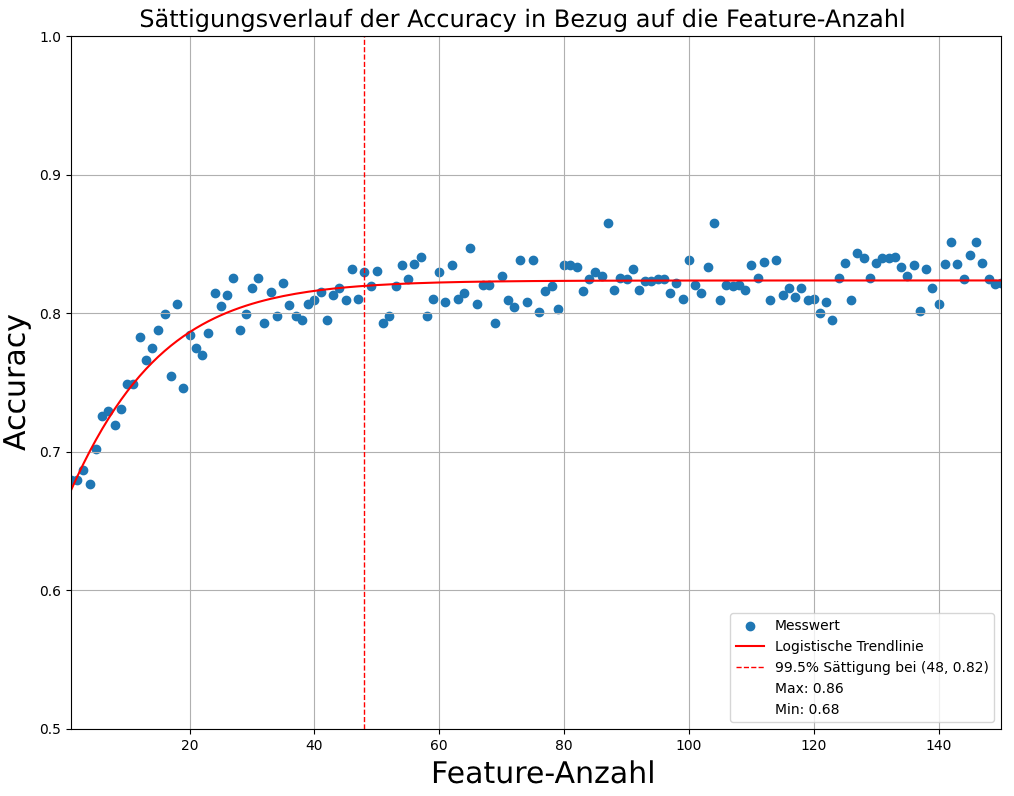
\includegraphics[width=0.9\textwidth]{img/Plots/bsp Accuracy verlauf.png}
    \caption[Beispiel eines Verlaufs der Accuracy in Bezug auf die Feature-Anzahl.]{Beispiel eines Verlaufs der Accuracy in Bezug auf die Feature-Anzahl, für die Feature-Vorauswahl. Die Accuracy verläuft in eine Sättigung.}
    \label{fig:bspSättAccu}
\end{figure}

Die resultierende Betrachtung, lässt eine grafische Beurteilung der Feature-Auswahl zu. Auch multivariate Einflüsse werden hier betrachtet. Jedoch ist das vorgehen noch modellabhängig. Um die Ergebnisse zu verallgemeinern, wird der Verlauf der Accuracy für jedes Modell in der Vorauswahl gemessen. Die Werte werden anschließend gemittelt. Dadurch entsteht ein Verlauf der Accuracy, welcher sich nicht auf ein bestimmtes Modell bezieht. Die Methode ist also verwendbar, um eine Feature-Rangfolge möglichst modellunabhängig zu Beurteilen.\par

Wichtig zu Erwähnen ist, dass die Featurewerte für eineiige Modelle skaliert werden müssen, damit diese mit den Features Arbeiten können. Für die lineare Regression werden diese auf den Wertebereich [0;1] skaliert. Für die SVMs werden alle Features auf den Wertebereich [-1;1] skaliert.\par

Wie in der Abbildung \ref{fig:bspSättAccu} zu sehen ist, läuft die Genauigkeit in eine Sättigung. Ein solcher Verlauf zeigte sich allen durchgeführten Versuchen. Da die Messwerte schwanken, wird der Verlauf mit einer Sättingungslinie approximiert. Somit steht ein stabileres Maß für die Beurteilung und für Vergleiche zur Verfügung. Der Sättigungsverlauf deutet auf Redundanzen in den Features hin. Ab einer bestimmten Feature-Menge erhält das Modell keine neuen Informationen durch mehr Features. Das ist nicht verwunderlich, da alle Features auf den 38 Basis-Features aufbauen. Der Sättigungsverlauf ist praktisch für die Feature-Auswahl, da über den Punkt ab dem die Sättigung erreicht wird, eine optimale Feature-Menge bestimmt ist. \par

Da die Rangfolge der Filter-Methoden wie bereits erwähnt, durch eine univariate Beurteilung erfolgt, ist zu vermuten, dass sie nicht optimal ist. Eine Rangfolge, welche die Features multivariat beurteilt ist wünschenswert. Mit den Wrapper Methoden lassen sich Features auswählen, mit einem Verfahren was auch multivariate Zusammenhänge verücksichtigt. Die Wrapper Methoden erstellen jedoch keine Rangfolge. Es werden deshalb unterschiedliche Messreihen mithilfe der Wrapper Methoden aufgenommen. Die Ergebnisse der Messreihen sollen in eine Rangfolge der Features überführt werden.\par

Aus der Anwendung der Wrapper Methoden auf ein Modell und eine Feature-Menge ist eine binäre Wertung eines Features abzuleiten: \textit{Ausgewählt} oder \textit{nicht Ausgewählt}. Werden mehrere Wiederholungen durchgeführt in denen die Wrapper Methoden angewendet werden, bei denen die Zusammensetzung der Feature-Menge variiert wird und auch das Modell, so entstehen mehrere binäre Evaluationen eines Features. Aus diesen kann eine Gesamtwertung des Features abgeleitet werden. Die Tabelle \ref{tab:bspWrapScore} veranschaulicht dies an einem Beispiel und die Formel \ref{eq:Meth WrapperScore} zeigt die Berechnung der Wertung.

\begin{table}[htb]
    \centering
    \caption{Beispiel einer Versuchsreihe zu dem Feature i, durch die Anwendung von Wrapper Methoden.}
    \begin{tabular}{|c|r|r|}
        \hline
        \multicolumn{3}{|r|}{\(Feature_i\)} \\
        \hline
        Versuch ID & Ausgewählt & Nicht Ausgewählt \\
        \hline
        0 & 1 & 0 \\
        1 & 1 & 0 \\
        2 & 0 & 1 \\
        3 & 1 & 0 \\
        4 & 0 & 1 \\
        5 & 1 & 0 \\
        \hline
        \hline
        Gesamt & 4 & 2 \\
        \hline
    \end{tabular}
    \label{tab:bspWrapScore}
\end{table}

\begin{equation}
W(x) = \frac{|\text{Ausgewählt}(x)|}{|\text{Ausgewählt}(x)| + |\text{Nicht Ausgewählt}(x)|} \rightarrow W(Feature_i)=\frac{4}{4+2} = 67\ \%
\label{eq:Meth WrapperScore}
\end{equation}

In der Formel \ref{eq:Meth WrapperScore} ist \(W(x)\) die Wertung eines Features \(x\). Zur Klarheit wird \(w\) im folgenden als \textit{Wrapper-Score} bezeichnet. Der Mechanismus der Wrapper-Score ist einfach. Wird ein Feature auch in unterschiedlichen Feature-Mengen und von unterschiedlichen Modellen oft ausgewählt, steigt der Wert. Das Maximum ist 1 und das Minimum 0. Features die in Kombination miteinander informativ sind, werden in der Hinsicht berücksichtigt, dass diese einen ähnlichen Wrapper-Score erzielen sollten. Sind sie sehr informativ, stehen sie gemeinsam weit oben in der Rangfolge. \par

Um eine aussagekräftige Rangfolge durch die Wrapper-Scores zu erhalten sind Messreihen aufzunehmen. Dazu sind mehrere Modelle zu benutzen. Verwendet werden eine klassische logistische Regression, eine lineare SVM und ein Random Forest Modell, ein Histogramm basiertes Gradient Boosting und eine polynomiale SVM. Die polynomiale SVM kann eine polynomiale Entscheidungsebene modellieren. Sie ist auf ein Polynomfunktion dritter Ordnung eingestellt. Die Feature-Mengen werden variiert, indem unterschiedliche Kombinationen der Oberkategorien der Features (\autoref{tab:FeatureMenge}) in die Modelle gegeben werden. Eine Variation der Zusammensetzung der Feature-Menge durch zufälliges Ziehen aus der Gesamtmenge, würde mehr Varianz bringen, jedoch ist das durchführen der Versuche zeitaufwändig. Um zu garantieren, dass jedes Feature betrachtet wird in einer praktikablen Zeit, wird sich für den beschriebenen Ansatz entschieden.\par

Wie in \autoref{sec:ML FeatSelect} beschrieben, gibt es mehrere Verfahren Wrapper-Methoden anzuwenden. Um auch hier für Varianz zu sorgen werden Messreihen aufgenommen mit der Vorwärtsauswahl und der Rückwärtsauswahl. Auch die Kriterien, nach denen Ausgewählt wird, werden variiert. In einigen Messreihen soll eine bestimmt Anzahl an Features von den Wrapper Methoden ausgewählt werden und in anderen Messreihen, sollen so viele Features ausgewählt werden bis die Performance nicht mehr steigt. Eine Übersicht über die durchgeführten Versuche befindet sich im Anhang. Sind bestimmte Versuche nicht mit bestimmten Feature-Kategorien, oder Modellen durchgeführt worden, lag dies am Rechenaufwand. Insgesamt wurden 179 unterschiedliche Kombinationen von Feature-Mengen, Wrapper-Methoden und Modellen getestet. \par

Aus diesen Versuchen lässt sich für jedes Feature ein Wrapper-Score ermitteln und eine Rangfolge der Features ist erstellbar. Diese Rangfolge kann modellunabhängig evaluiert werden, über den Plot der Accuracy, wie in \autoref{fig:bspSättAccu}. \par

Prädestiniert für Redundanz sind Features, die sich die gleiche Basis teilen. Wie zum Beispiel die maximale Geschwindigkeit einer Trajektorie, welche einmal in ihrer Basisform vorliegt und auch in Perzentile eingeteilt. Ist eine Feature-Basis sehr informativ, ist es nicht unwahrscheinlich, dass mehrere Features, die sich diese Basis teilen einen hohen Rang erzielen und Redundanz entsteht in der Feature-Auswahl. Um das zu reduzieren, wird lediglich das höchstrangige Feature der gleichen Basis in der Rangfolge behalten. Features mit gleicher Basis, aber niedrigeren Rang werden aus der Rangfolge entfernt. Interaktionsfeatures stellen dabei ihre eigene Basis dar. Die Kombination aus maximaler Geschwindigkeit und der mittleren Objektanzahl teilt sich bei dieser Methode nicht die gleiche Basis wie die maximale Geschwindigkeit und auch nicht wie die mittlere Objektanzahl. Anderes gilt für die Interaktion mit sich selbst. \par

Die Evaluation bestätigt, dass durch das Eliminieren von Features mit gleicher Basis eine effizientere Rangfolge entsteht. Die Sättigung wird früher erreicht. In \autoref{sec:Ergeb FeatSel,Hyp,ModSel} wird dies genauer dargestellt. \par

Abschließend wird untersucht, ob alle Feature-Kategorien benötigt werden. Dazu werden aus der Rangfolge nur Features aus bestimmten Kategorien genommen und evaluiert. Im Anhang befindet sich eine tabellarische Übersicht über die durchgeführten Versuche. \par

Bei der Auswertung in \autoref{sec:Ergeb FeatSel,Hyp,ModSel} zeigt sich, dass mit der Zusammensetzung der Feature-Menge aus Basis-Features, Interaktionsfeatures und Quantil-Features die besten Ergebnisse erzielt werden. Die Box-Cox-Features und die Logarithmus-Features werden aus der Vorauswahl herausgenommen. \par

Mit der resultierenden Rangfolge wird mit 29 Features die Sättigung der Accuracy erreicht. Um die Menge der Features in der Vorauswahl nicht zu sehr zu beschneiden, werden die besten 150 Features der Rangfolge als Vorauswahl genommen. 



\subsection{Einstellung der Hyperparameter} \label{sec:Meth HyperparaKonf}
Für die zur Auswahl stehenden Modelle sind passende Hyperparameter zu finden. Dafür verwendet werden die 150 Features der Vorauswahl. Für die Hyperparametersuche wird eine Random Search durchgeführt (\autoref{sec:ML HyperPara}). Versuche die Methode der Grid Search anzuwenden zeigten, dass diese zu viel Rechenzeit benötigt. Eingestellt werden die folgenden Modelle.

\begin{enumerate}
    \item Logistische Regression
    \item Lineare SVM
    \item Polynomiale SVM
    \item Random Forest
    \item Gradient Boosting
    \item Histogramm basiertes Gradient Boosting
\end{enumerate}

Insgesamt werden für jedes Modell 500 Kombinationen von Hyperparametern getestet. Diese werden mittels Cross-Validation beurteilt. Da in vorherigen Tests bemerkt wurde, dass die Accuracy schwanken kann, wurde jede Kombination 150 mal Validiert. Das scheint möglicherweise etwas exzessiv, jedoch ist das Ziel bei diesem Vorgehen, eine statistische Stabilität der Accuracy zu erhalten. Nur wenn diese gegeben ist, kann der Aussage vertraut werden, dass eine bestimmt Kombination an Hyperparametern besser ist als eine Andere. Die Schwankungen in der Accuracy sind vermutlich auf die geringe Datenmenge zurückzuführen. \par

Um die hohe Anzahl an Validierungswerten zu erhalten, wird eine mehrfache Cross-Validation durchgeführt. Insgesammt wird der Trainingsdatensatz in 10 Teile zerteilt mit denen jeweils eine Validierung durchgeführt wird. Anschließend wird der Trainingsdatensatz erneut in andere 10 Teile zerteilt, damit die Daten wieder gemischt werden. Anschließend wird erneut Validiert. Dies wird insgesamt 15 mal wiederholt. \par

Die erzielte Accuracy und die dazugehörigen Hyperparameter werden abgespeichert. Nach Vollendung der Random Search können die Ergebnisse in eine Reihenfolge gebracht werden. Die Hyperparameter, mit denen die beste Performance erzielt wurde, werden für das Modell übernommen. \par

Informativ kann auch die Betrachtung der Hyperparameter der oberen Ränge sein, da diese ebenfalls eine hohe Accuracy erzielten. Hyperparameter in den oberen Rängen, welche sich immer in ähnlichen Größenordnungen befinden, sind mit hoher Sicherheit gut eingestellt. Schwanken die Werte eines Hyperparameters stark, dann ist dieser entweder nicht relevant für die Lösung der Aufgabe, oder es herrschen Mehrdeutigkeiten in der Kombination mit anderen Hyperparametern. \par

Eine ausführliche Übersicht über die Hyperparameter der einzelnen Modelle und die Wahrscheinlichkeitsverteilungen, aus denen die Random Search die jeweilgen Paramterwerte zieht befindet sich im Anhang. 

\subsection{Auswahl des Modells und der Features}\label{sec:Meth ModelSele}
Da nun die Modelle eingestellt sind und eine Feature Vorauswahl vorhanden ist, ist die finale Entscheidung für ein Modell einfach. Für jedes eingestellte Modell wird der Verlauf der Accuracy im Bezug auf die Rangliste ermittelt, wir in \autoref{fig:bspSättAccu} beispielhaft dargestellt. Anschließend können die Verläufe vergleichen werden. Das Modell, welches die beste Performance zeigt, wird ausgewählt. Über den Sättigungspunkt ist eine optimale Feature-Menge direkt ablesbar. Erzielen zwei Modelle die gleiche Performance, wird das Modell bevorzugt, welches diese mit der geringsten Feature-Menge erreicht. \par

Es zeigt sich, dass eine polynomiale SVM das beste Modell ist. Die Entscheidungsebene ist mit einer Funktion zweiten Grades modellierbar. Der Sättigungspunkt wird laut Trendlinie mit 18 Features erreicht, um für mehr Stabilität tiefer in der Sättigung zu liegen, werden die besten 40 Features verwendet. Die polynomiale SVM implementiert keine Embedded-Methoden für die Feature-Auswahl, somit wird die Auswahl nicht weiter Optimiert. \par

Abschließend wird das Modell trainiert und getestet. Der Test bestätigt Modell, wie in \autoref{sec:Ergeb ModEntwi} dargestellt wird.\par

Im Anhang befindet sich eine Liste der ausgewählten Features. Ebenfalls sind dort die ermittelten Hyperparameter des finalen Modells tabellarisch dargestellt.